\part{Cicli inversi}
\begin{adjustwidth}{2in}{}
	L'effetto utile di un ciclo inverso, piuttosto che la produzione lavoro, è la produzione di un effetto frigorifero, ovvero la sottrazione di una potenza termica da un ambiente più freddo ad un ambiente più caldo "violando" il corso naturale degli eventi: ciò infatti è possibile solamente fornendo un'azione compensatrice sotto forma di energia, che può essere 
	\begin{itemize}
		\item \textbf{Meccanica}: macchine frigorifere a compressione di calore
		\item \textbf{Termica}: macchine frigorifere ad assorbimento
	\end{itemize}
	Tale ciclo può essere utilizzato sia per raffreddare che per riscaldare ambienti attraverso la pompa di calore. 		
\begin{figure}[H]
	\centering
	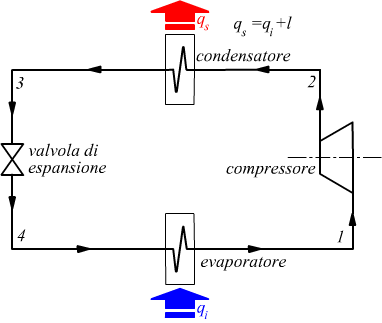
\includegraphics[width=0.4\linewidth]{immagini/cicliinversi}
	\label{fig:cicliinversi}
\end{figure}
	Il compressore è l'organo incaricato all'immissione del lavoro all'interno del ciclo, generalmente è di tipo volumetrico-alternativo, ciò significa all'entrata del compressore, per non danneggiare pistoni e cilindro, è necessario immettere vapore leggermente surriscaldato, perché nel caso ci fosse liquidi - per sua natura incomprimibile - si concentrerebbe sul volume morto e causerebbe problemi all'organo. 
	
	Il fluido esce dal compressore come vapore surriscaldato, dopodiché raggiunge il condensatore, questo è uno scambiatore di calore che si occupa di rilasciare calore verso l'ambiente. il fluido esce dal condensatore il condizioni di liquido saturo ed entra in una valvola di laminazione, che attraverso una trasformazione adiabatica di laminazione (isoentalpica), riporta il fluido alla pressione iniziale, a questo punto all'interno di un evaporatore assorbirà calore dall'ambiente e si ricondurrà nuovamente al compressore.
	
	Similmente agli impianti a vapore, poiché l'impianto è operativamente prossimo alle condizioni critiche, non si possono utilizzare le relazioni dei gas perfetti ma apposite tabelle dei liquidi refrigeranti. \newline 
	
	Sui diagrammi di interesse un ciclo frigorifero diviene 
\end{adjustwidth}		
\begin{figure}[H]
	\centering
	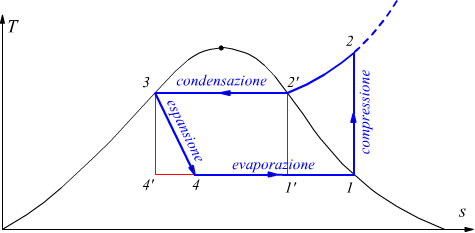
\includegraphics[width=0.4\linewidth]{immagini/cicliinversi1}
	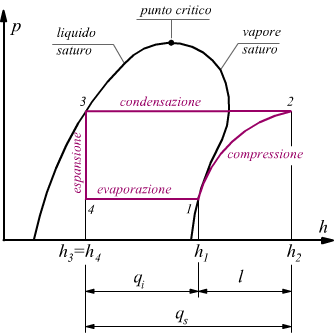
\includegraphics[width=0.4\linewidth]{immagini/cicliinversi2}
	\label{fig:cicliinversi1}
\end{figure}
\begin{adjustwidth}{2in}{}
	Come funziona un ciclo frigorifero? 
	
	La temperatura di passaggio di fase dipende dalla pressione,  comprimendo si alza la temperatura a cui avviene il passaggio di fase, per cui col compressore si porta la pressione superiore ad un livello tale per cui la temperatura di condensazione  sia almeno di 5 0 10 gradi superiore a quella esterna cosicché si possa condensare e quindi rilasciare calore all'ambiente esterno.
	
	Dopodiché espandendo all'interno della valvola di laminazione si ritorna alla pressione più bassa che corrisponde ad una temperatura di evaporazione di 5 o 10 gradi più bassa rispetto alla temperatura dell'ambiente da refrigerare. \newline 
	
	Nel caso in cui invece si utilizzasse questo sistema come pompa di calore l'effetto utile sarà dato dal condensatore, ovvero da quanta energia termica si riuscirà ad immettere nell'ambiente per riscaldarlo: rispetto al caso frigorifero si invertono così temperatura dell'utenza (ovvero quella dell'ambiente da condizionare, che ora è più alta) e la temperatura dell'ambiente esterno (che ora è più bassa) ma la macchina rimane la stessa e il ciclo rimane invariato, cambia soltanto l'effetto utile.\newline 
	
	Infatti per i cicli inversi, piuttosto che il rendimento si definisce il coefficiente di prestazione COP
	\[COP = \dfrac{\text{effetto utile}}{\text{energia spesa}}>1\]
	L'"efficienza" in questo tipo di cicli è maggiore dell'unità perché si sta convertendo lavoro (energia di prima specie, nobile, che può essere convertito in ogni forma di energia) in calore (energia di seconda specie, meno nobile).\newline 
	
	Per un ciclo frigorifero
	\[COP_f = \dfrac{Q_{41}}{L_{12}} = \dfrac{h_1-h_4}{h_2-h_1} = 2\div4\]
	Il range di valori è fortemente dipendente dalle condizioni operative, infatti tanto più cresce il $\Delta T$, tanto più si dovrà comprimere e tanto più il COP diminuirà.\newline 
	
	Per un ciclo pompa di calore 
	\[COP_{PdC} = \dfrac{Q_{23}}{L_{12}} = \dfrac{Q_{41} + L_{12} }{L_{12}} =COP_f + 1 = 3\div5\]
	
	Importante è la distinzione tra la temperatura dell'ambiente esterno $T_{amb}$ e la temperatura dell'utenza, ovvero quella dell'ambiente da condizionare $T_u$: il ciclo deve svolgersi sempre all'esterno di queste due temperature, l'evaporatore deve poter sempre assorbire calore ed il condensatore deve poter sempre cedere calore.
	
	Deve perciò esistere sempre un $\Delta T$ (lo stesso) tra la temperatura dell'ambiente e quella del condensatore e tra la temperatura dell'utenza e quella dell'evaporatore (Frigorifero); e tra la temperatura dell'ambiente e quella dell'evaporatore e tra la temperatura dell'utenza e del condensatore (Pompa di Calore).  
\end{adjustwidth}




\section{Variazione del ciclo base}
\subsection{Rigenerazione}
\begin{adjustwidth}{2in}{}
	
	DISEGNO
	
	Aggiungendo uno scambiatore intermedio che metta in contatto il fluido in uscita dal condensatore con quello in ingresso al compressore, si aggiungono 2 trasformazioni:
	\begin{itemize}
		\item \textbf{61} di preriscaldamento del vapore che andrà compresso
		\item \textbf{34} di raffreddamento del vapore che andrà laminato. 
		
		Queso in particolare giova al ciclo perché diminuendo il titolo del punto di inizio evaporazione (5) si aggiunge una parte di evaporazione in più e quindi sia aumenta l'effetto utile che è possibile trarre dal sistema. 
		\[COP = \dfrac{h_6-h_5}{h_2-h_1}\]
	\end{itemize} 
\end{adjustwidth}

\subsection{Interrefrigerazione}
\begin{adjustwidth}{2in}{}
	Per compiere un ciclo frigorifero com un grande $\Delta T$, dato che il lavoro di compressione sarebbe troppo elevato e sconveniente, si passa attraverso l'interrefrigerazione. 
	
	Si uniscono ciò due cicli a cascata mediante un serbatoio intermedio che raffredda il vapore che esce dal primo compressore e consente di frazionare la linea di espansione.
	
	DISEGNI
	
	La presenza del separatore intermedio consente di comprimere da 1 a 2 e raffreddare fino a 3 ripescando il vapore saturo e poi di ricomprimere fino a 4: ciò consente di risparmiare lavoro perché il punto di fine compressione, se questa non fosse stata frazionata, sarebbe stato in A.
	
	Un altro vantaggio è che alla pressione intermedia, tramite il separatore, si ripesca solamente liquido saturo in 7 e quindi si inizia ad evaporare al punto 8, se invece sia avesse espanso in una sola trasformazione a partire a 5, il punto di inizio evaporazione sarebbe stato B, e dato che $x_B>x_8$ con un effetto utile più ristretto. 
	
	In sostante il ciclo interrefrigerato porta con se du vantaggi: sulla compressione e sulla produzione di effetto utile. \newline 
	
	Questo schema prevede poi che la portata che fluisce nella zona superiore sia diversa da quella che fluisce nella zona inferiore, perché avvenendo in 6 la separazione, significa che nel punto 7 si prende solamente il liquido all'interno del separatore. 
	
	Come si determina il rapporto tra le due portate? Attraverso il bilancio termico al separatore
	\[\dot{m}_{cond}h_6 + \dot{m}_{evap}h_2 = \dot{m}_{cond}h_3 + \dot{m}_{evap}h_3 \]
	Allora 
	\[\Phi = \dfrac{\dot{m}_{cond}}{\dot{m}_{evap}} = \dfrac{h_2-h_7}{h_5-h_6}\]
	La potenza all'evaporatore sarà così calcolabile come 
	\[P_{evap} = \dot{m}_{evap}(h_1-h_8)\]
	Ed il COP sarà conseguentemente pari a 
	\[COP = \dfrac{Q_81}{L_{12}+L_{34}} = \dfrac{\dot{m}_{evap}(h_1-h_8)}{\dot{m}_{evap}(h_2-h_1) + \dot{m}_{cond}(h_4-h_3)} = \dfrac{h_1-h_8}{h_2-h_1 + \Phi(h_4-h_3)}\]
	Con questi tipi di impianti si può arrivare anche a $\Delta T \approx 60\degree C$.
\end{adjustwidth}





\section{Fluidi refrigeranti}
\begin{adjustwidth}{2in}{}
	Un fluido frigogeno dovrebbe avere
	\begin{itemize}
		\item \textbf{Alta temperatura critica}, al di sopra della temperatura di condensazione che si realizza nel ciclo. 
		\item \textbf{Bassa temperatura di solidificazione} in modo da non solidificare nelle normali condizioni di funzionamento
		\item \textbf{Alto calore di vaporizzazione} così da produrre un elevato effetto frigorifero
		\[P_{evap} = \dot{m}x\Delta h\]
		Crescendo $\Delta h$ - a potenza costante - diminuisce la portata e ciò consente di avere sezioni di passaggio più piccole e quindi macchine più compatte. 
		\item \textbf{Pressioni di esercizio} più \textbf{basse} possibili \textbf{ma superiori a quella atmosferica}, in questo modo oltre ad evitare costruzioni pesanti e costose si evitano infiltrazioni di aria nell'impianto
		\item \textbf{Chimicamente inerte}
		\item \textbf{Bassa potenzialità di distruzione dell'ozono e di effetto serra}
	\end{itemize}
	Tra i fluidi proposti possiamo individuare
	\begin{itemize}
		\item $H_2O$: inutilizzabile sotto gli 0 \degree C
		\item $CO_2, CH_3CH_2CH_3 (\text{propano})$: dalle caratteristiche termodinamiche poco convincenti
		\item $NH_3$: esplosivo se miscelato con $O_2$
		\item \textbf{Fluidi frigoneni alogenati}\\
		Non tossici, non infiammabili, non corrosivi, dalle ottime proprietà termodinamiche. 
		
		Questi vengono prodotti in maniera sintetica attraverso la sostituzione di un idrogeno con un cloro o un fluoro. \newline 
		
		La nomenclatura segue questa regola 
		\[R-MNP = C_{M+1}H_{N-1}Cl_xF_p\]
		Il fluido più comune è l'R134 (o HFC-134a o 1,1,1,2-tetrafluoroetano) la cui formula sarà
		\[C_2H_2F_4\]
		Tra questi tipo di fluidi si possono trovare 
		\begin{itemize}
			\item \textbf{CFC}: clorofluorocarburi
			\item \textbf{HCFC}: idroclorofluorocarburi\\
			
			Entrambi sono responsabili del buco dell'ozono, il Cloro catalizza la trasformazione  $O_3 \rightarrow O_2$
			
			\item \textbf{HFC}: idrofluorocarburi
			\item \textbf{FC}: fluorocarbuti\\
			
			Tutte e quattro le tipologie, se disperse in atmosfera, contribuiscono all'effetto serra.
		\end{itemize}
	\end{itemize}
\end{adjustwidth}


\newpage


\section{Macchine frigorifere ad assorbimento}
\begin{adjustwidth}{2in}{}
	Un'altra forma di energia che si può usare in input al ciclo è quella termica: in questo modo nascono le macchine frigorifere ad assorbimento.
	
	DISEGNO
	
	Si sostituisce il compressore con un'altra linea d'impianto e la pompa (ex compressore) ora elabora liquido piuttosto che gas e quindi richiede un lavoro specifico minore. \newline 
	
	Il principio di funzionamento si basa sulla solubilità dei fluidi, ovvero esiste un liquido assorbitore ed un liquido frigorifero che si possono miscelare, entrare in soluzione.
	
	Nel generatore si fornisce una potenza termica ad elevata temperatura cosicché da questa soluzione evapori il fluido frigorifero in modo da convogliarlo nel resto dell'impianto affinché assolva le sue funzioni quindi passare verso il condensatore, alla valvola  e all'evaporatore, dopo di ciò il vapore di fluido frigorifero incontrerà nell'assorbitore la soluzione di liquido assorbente e liquido frigorifero scarica di liquido frigorifero, in uscita dal generatore, in modo che il fluido frigorifero rientri di nuovo in soluzione liberando una certa potenza termica; a questo punto attraverso una pompa si aumenta la pressione della soluzione che viene reinviata al generatore. 
	
	Poiché il generatore si trova tra i $100\div130$\degree C e l'assorbitore è a temperatura ambiente, si può inserire un recuperatore che riscaldi il fluido al generatore e raffreddi il fluido all'assorbitore, in questo modo si riduce l'energia spesa $Q_G$. \newline 
	
	Le principali coppie di fluidi utilizzate sono		
\begin{itemize}
		\item $H_2O$: assorbitore - $NH_3$: refrigerante
		\item $BrLi$: assorbitore - $H_2O$: refrigerante per $T_u>0\degree C$
\end{itemize}
	Si definiscono anche qui 
	\[COP_f = \dfrac{Q_E}{Q_G}\]
	\[COP_{PdC} = \dfrac{Q_C-Q_A}{Q_G} = \dfrac{Q_G-Q_A}{Q_G} = COP_f+1\]
	
	Questi impianti vengono definiti tritermici, perché sussistono tre livelli di temperatura
	\[T_G = 1--\div130\degree C ~~T_{amb}\approxeq T_{cond} \approxeq T_A ~~> T_{evap} \approx T_u \]
\end{adjustwidth}


\newpage


\subsection{Studio del processo ideale}
\begin{adjustwidth}{2in}{}
	Si suddivida il processo in due sottoprocessi attraverso l'utilizzo di pozzi termici, tra la temperatura ambiente, quella dell'utenza e quella del generatore.
	
	DISEGNO
	
	In prima istanza si immagini la presenza di una macchina motrice di Carnot che assorbe la potenza termica alla temperatura più elevata e produce lavoro rilasciando calore all'ambiente per mezzo dell'assorbitore.
	 
	Si immagini poi una seconda macchina frigorifera di Carnot che riceva in ingresso sia il lavoro prodotto dalla macchina motrice di Carnot, che il calore dell'evaporatore e rilasci calore all'ambiente per mezzo dell'assorbitore.
	
	Allora è possibile scrivere, per la macchina motrice di Carnot
	\[\eta^* = \dfrac{L}{Q_G} = 1 - \dfrac{T_A}{T_G} \Rightarrow L = Q_G\left(1-\dfrac{T_A}{T_G}\right)\]
	Mentre per la macchina frigorifera di Carnot
	\[COP^* = \dfrac{Q_E}{L} = \dfrac{T_u}{T_A-T_u} \Rightarrow Q_E = L\dfrac{T_u}{T_A-T_u} = Q_G\dfrac{T_G-T_A}{T_G}\dfrac{T_u}{T_A-T_u} \]
	Allora il massimo COP aspirabile per una macchina reale sarà 
	\[COP_{\max} = \dfrac{Q_E}{Q_G} = \dfrac{T_G-T_A}{T_G}\dfrac{T_u}{T_A-T_u}\approx [1\div2]\]
	L'energia che ora si immette in ingresso è calore e non più lavoro: si sta convertendo energia di seconda specie in energia di seconda specie, il rendimento è sempre maggiore dell'unità ma minore del ciclo a compressione di vapore, se infatti si aumenta la nobilità dell'energia termica fornita aumentando la temperatura, ci si può avvicinare al rendimento del COP a vapore. \newline 
	
	I principali vantaggi che si possono sfruttare del ciclo ad assorbimento sono 
	\begin{itemize}
		\item Recupero di calore dispero dai processo industriali
		\item Piccoli impianti vicino all'utenza che recuperano il calore di scarto della grandi centrali termoelettriche (es. teleriscaldamento)
	\end{itemize}
\end{adjustwidth}

